%! alt Trapezium ABCD with AB = 4 at the top and CD = 6 at the bottom. The diagonals of ABCD meet at a point on the highlighted segment l2, of length 24/5, which runs between the legs AD and BC parallel to AB. The diagonals of the trapezium with parallel sides CD and l2 meet on l3, of length 16/3, and the diagonals of the trapezium with parallel sides l2 and l3 meet on l4. Each new segment lies between the two before it, so the segments close in on one limiting segment.
%! after_paragraph 1
%! scale 13/10
% The shared preamble of every Cevian figure. pipeline/figures turns these colours into theme-aware paint,
% and refuses any other colour, so draw only with them:
%   figink (lines and labels), figaux (construction lines), figaccent (the object the argument turns on),
%   figtint and figaccenttint (light fills).
\documentclass[border=1.5pt]{standalone}
\usepackage{tkz-euclide}
\definecolor{figink}{RGB}{0,0,0}
\definecolor{figaux}{RGB}{85,85,85}
\definecolor{figaccent}{RGB}{192,57,43}
\definecolor{figtint}{RGB}{221,221,221}
\definecolor{figaccenttint}{RGB}{245,213,208}
% tkz-euclide's defaults draw circles, compasses and marks in 50% grey and fill points with a tint.
\makeatletter
\def\tkz@otherlinecolor{figink}
\def\tkz@euc@circlecolor{figink}
\def\tkz@euc@compasscolor{figink}
\def\tkz@euc@mkcolor{figink}
\def\tkz@mk@fill{figink}
\def\tkz@euc@pointfillcolor{figink}
\makeatother
\tkzSetUpLine[color=figink,line width=.7pt]
\tkzSetUpArc[color=figink,line width=.7pt]
\tkzSetUpCompass[color=figink,line width=.5pt]
\tkzSetUpPoint[color=figink,fill=figink,size=3.1pt]
\tikzset{
  every picture/.style={line cap=round,line join=round,color=figink},
  circle style/.append style={color=figink,line width=.7pt},
  aux/.style={color=figaux,line width=.45pt,dash pattern=on 2.6pt off 2pt},
  key/.style={color=figaccent,line width=1pt},
  mk/.style={color=figink,line width=.5pt},
  lbl/.style={color=figink,inner sep=2.2pt},
  len/.style={color=figink,inner sep=1.5pt,font=\small},
}

\begin{document}
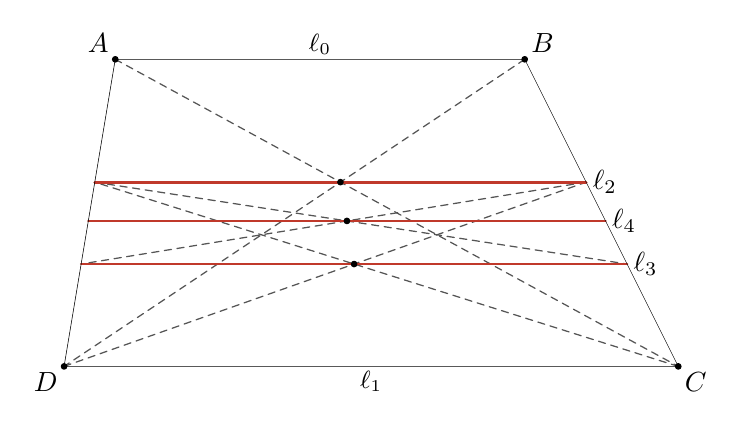
\begin{tikzpicture}
\tkzDefPoint(0.0,0.0){D} %! D = (0, 0)
\tkzDefPoint(7.8000000,0.0){C} %! C = (6, 0)
\tkzDefPoint(0.65000000,3.9000000){A} %! A = (1/2, 3)
\tkzDefPoint(5.8500000,3.9000000){B} %! B = (9/2, 3)
\tkzDefPoint(3.5100000,2.3400000){Oa} %! Oa = meet(A, C, B, D)
\tkzDefPoint(0.39000000,2.3400000){Pb} %! Pb = meet(Oa, shift(Oa, 1, 0), A, D)
\tkzDefPoint(6.6300000,2.3400000){Qb} %! Qb = meet(Oa, shift(Oa, 1, 0), B, C)
\tkzDefPoint(3.6833333,1.3000000){Ob} %! Ob = meet(D, Qb, C, Pb)
\tkzDefPoint(0.21666667,1.3000000){Pc} %! Pc = meet(Ob, shift(Ob, 1, 0), A, D)
\tkzDefPoint(7.1500000,1.3000000){Qc} %! Qc = meet(Ob, shift(Ob, 1, 0), B, C)
\tkzDefPoint(3.5921053,1.8473684){Oc} %! Oc = meet(Pb, Qc, Qb, Pc)
\tkzDefPoint(0.30789474,1.8473684){Pd} %! Pd = meet(Oc, shift(Oc, 1, 0), A, D)
\tkzDefPoint(6.8763158,1.8473684){Qd} %! Qd = meet(Oc, shift(Oc, 1, 0), B, C)
%! fact dist(A, B) == 4
%! fact dist(C, D) == 6
%! fact parallel(A, B, D, C)
%! fact dist(Pb, Qb) == 24/5
%! fact dist(Pc, Qc) == 16/3
%! fact parallel(Pb, Qb, A, B)
%! fact parallel(Pc, Qc, A, B)
%! fact parallel(Pd, Qd, A, B)
%! fact collinear(Oa, Pb, Qb)
%! fact collinear(Ob, Pc, Qc)
%! fact collinear(Oc, Pd, Qd)
%! fact equal(dist(Pb, Qb), 2 * dist(A, B) * dist(C, D) / (dist(A, B) + dist(C, D)))
%! fact equal(dist(Pc, Qc), 2 * dist(C, D) * dist(Pb, Qb) / (dist(C, D) + dist(Pb, Qb)))
%! fact equal(dist(Pd, Qd), 2 * dist(Pb, Qb) * dist(Pc, Qc) / (dist(Pb, Qb) + dist(Pc, Qc)))
%! example dist(Pd, Qd) == 96/19
\tkzDrawSegments[aux](A,C B,D D,Qb C,Pb Pb,Qc Qb,Pc)
\tkzDrawSegments[key](Pb,Qb Pc,Qc Pd,Qd)
\tkzDrawPolygon(A,B,C,D)
\tkzDrawPoints(A,B,C,D,Oa,Ob,Oc)
\tkzLabelPoint[above left,lbl](A){$A$}
\tkzLabelPoint[above right,lbl](B){$B$}
\tkzLabelPoint[below right,lbl](C){$C$}
\tkzLabelPoint[below left,lbl](D){$D$}
\tkzLabelSegment[above,len](A,B){$\ell_0$}
\tkzLabelSegment[below,len](D,C){$\ell_1$}
\tkzLabelPoint[right,lbl](Qb){$\ell_2$}
\tkzLabelPoint[right,lbl](Qc){$\ell_3$}
\tkzLabelPoint[right,lbl](Qd){$\ell_4$}
\end{tikzpicture}
\end{document}
